\section{Annihilating the Steinberg kernel}\label{sec:kernel}

The affine group of Section~\ref{sec:affine} uses a Steinberg group,
whose matrix action can have a kernel.  We now show that the coefficient
endomorphism annihilates this entire kernel. The argument uses the
splitting pairs from Theorem~\ref{thm:algebra-package}, whose elements
commute with the coefficient image.
It is convenient to state it for an arbitrary unital associative ring.

Recall that $\operatorname{St}_6(R)$ has generators $x_{ij}(a)$, where
$1\leq i\ne j\leq6$ and $a\in R$, with relations
\begin{align}
 x_{ij}(a)x_{ij}(b)&=x_{ij}(a+b),\label{eq:kernel-additive}\\
 [x_{ij}(a),x_{jk}(b)]&=x_{ik}(ab)
       &&(i,j,k\text{ distinct}),\label{eq:kernel-chain}\\
 [x_{ij}(a),x_{kl}(b)]&=1
       &&(i\ne l,\ j\ne k).\label{eq:kernel-distant}
\end{align}
Here $[u,v]=uvu^{-1}v^{-1}$.  Let
$\pi:\operatorname{St}_6(R)\to\operatorname{E}_6(R)$ send
$x_{ij}(a)$ to $I+ae_{ij}$.

\begin{theorem}\label{thm:kernel}
Let $R$ be a unital associative ring, let $\psi:R\to R$ be an additive
multiplicative map, and put $P=\psi(1)$.  Suppose that
$U_0,U_1,V_0,V_1\in PRP$ commute with $\psi(R)$ and satisfy
\[
 V_iU_j=\delta_{ij}P,\qquad U_0V_0+U_1V_1=P.
\]
Then the homomorphism
\[
 \theta:\operatorname{St}_6(R)\longrightarrow\operatorname{St}_6(R),
 \qquad x_{ij}(a)\longmapsto x_{ij}(\psi(a)),
\]
satisfies $\theta(\ker\pi)=1$.
\end{theorem}

For the binary Leavitt algebra $L=L_{\F_2}(1,2)$, Khanh proves that
the natural map $\St_r(L)\to\mathrm{GL}_r(L)$ is an isomorphism for
$r\ge3$ \cite[Theorem~5.4]{Khanh2026Leavitt}.
Theorem~\ref{thm:kernel} concerns an arbitrary ring and annihilation
of its matrix kernel under the specified coefficient map.

Additivity and multiplicativity make $\theta$ a homomorphism by the
defining relations.  The map $\psi$ need not preserve the identity.
For any additive
multiplicative map $\lambda:R\to R$, the corresponding image of a root
word with matrix $g$ has matrix
\begin{equation}\label{eq:kernel-nonunital}
 I+\lambda^{(6)}(g-I),
\end{equation}
where $\lambda^{(6)}$ acts entrywise.  This follows on generators and
then on products by expanding $gh-I=(g-I)+(h-I)+(g-I)(h-I)$.
In particular, coefficient maps preserve the condition of having
identity matrix.  We shall use this for maps whose images lie in
smaller idempotent corners of $R$.

The proof has two parts.  First, a word with identity matrix becomes
central when all its coefficients are placed in a suitable corner.
Second, two orthogonal copies of that corner can be interchanged and
split.  Four corners suffice to make the resulting central element
equal to its square.

\subsection{Conjugation with an unused index}

The use of an index outside the support of a root word is the classical
Steinberg centrality argument; see
\cite[proof of Theorem~III.5.2.1]{Weibel2013}.
We record its row-and-column form to justify the corner conjugations
inside the Steinberg group. The kernel-annihilation theorem also uses
the corner comparisons and four-corner splitting proved below.

\begin{lemma}\label{lem:external-roots}
Let $J\subseteq\{1,\ldots,6\}$ and $k\notin J$.  For a column $c$ and
a row $r$ indexed by $J$, put
\[
 C_k(c)=\prod_{i\in J}x_{ik}(c_i),\qquad
 R_k(r)=\prod_{i\in J}x_{ki}(r_i).
\]
If $w$ is a root word using only indices in $J$, and $A$ is its matrix
on those indices, then
\begin{equation}\label{eq:external-action}
 wC_k(c)w^{-1}=C_k(Ac),\qquad
 wR_k(r)w^{-1}=R_k(rA^{-1}).
\end{equation}
Consequently, an element represented by a root word omitting index $6$
and having identity matrix is central in $\operatorname{St}_6(R)$.
\end{lemma}

\begin{proof}
The factors in each defining product commute.  It suffices to check
conjugation by $x_{ij}(a)$ with $i,j\in J$.  Its only changed column
factor and row factor are, respectively,
\begin{align*}
 x_{ij}(a)x_{jk}(c_j)x_{ij}(a)^{-1}
    &=x_{ik}(ac_j)x_{jk}(c_j),\\
 x_{ij}(a)x_{ki}(r_i)x_{ij}(a)^{-1}
    &=x_{kj}(-r_i a)x_{ki}(r_i).
\end{align*}
The first identity is \eqref{eq:kernel-chain}.  For the second,
reverse the relation
$[x_{ki}(r_i),x_{ij}(a)]=x_{kj}(r_i a)$.
These operations are multiplication of a column by $I+ae_{ij}$ and
of a row by $I-ae_{ij}$.  Composition proves
\eqref{eq:external-action} inside the Steinberg group.

If $w$ omits $6$ and has identity matrix, it therefore commutes with
every $x_{i6}(a)$ and $x_{6i}(a)$.  It commutes with every remaining
root as well, since
\[
 x_{ij}(a)=[x_{i6}(a),x_{6j}(1)]\qquad(i,j\ne6).
\]
These roots generate the group.
\end{proof}

\begin{lemma}\label{lem:corner-centrality}
Let $E,F\in R$ be idempotents with $EF=FE=0$.  Suppose $d,d^*\in R$ satisfy
\begin{equation}\label{eq:corner-equivalence}
 d=FdE,\qquad d^*=Ed^*F,\qquad d^*d=E,\qquad dd^*=F.
\end{equation}
Every root word whose coefficients lie in $ERE$ and whose matrix is
the identity represents a central element of
$\operatorname{St}_6(R)$.
\end{lemma}

\begin{proof}
Here $d^*$ denotes the specified element in
\eqref{eq:corner-equivalence}; no involution on $R$ is assumed.  Put
\[
 W=x_{16}(d)x_{61}(-d^*)x_{16}(d).
\]
Its matrix and inverse on the ordered pair $(1,6)$ are
\begin{equation}\label{eq:corner-compression-matrix}
 H=\begin{pmatrix}1-F&d\\-d^*&1-E\end{pmatrix},\qquad
 H^{-1}=\begin{pmatrix}1-F&-d\\d^*&1-E\end{pmatrix}.
\end{equation}
These formulas follow by multiplying the three elementary matrices
and using \eqref{eq:corner-equivalence}.

Let $y=EyE$ and $k\notin\{1,6\}$.  Applying
Lemma~\ref{lem:external-roots} to the actual word $W$ gives
\begin{equation}\label{eq:corner-compression-roots}
 \begin{aligned}
 Wx_{1k}(y)W^{-1}&=x_{1k}(y),&
 Wx_{6k}(y)W^{-1}&=x_{1k}(dy),\\
 Wx_{k1}(y)W^{-1}&=x_{k1}(y),&
 Wx_{k6}(y)W^{-1}&=x_{k1}(yd^*).
 \end{aligned}
\end{equation}
Indeed $d^*y=yd=0$, since $E$ and $F$ are orthogonal, and
$(1-E)y=y(1-E)=0$.  Roots with both indices outside $\{1,6\}$
commute with $W$.

For the two roots internal to this pair, first write
\[
 x_{16}(y)=[x_{1k}(y),x_{k6}(E)],\qquad
 x_{61}(y)=[x_{6k}(y),x_{k1}(E)].
\]
Their conjugates under $W$ are, by
\eqref{eq:corner-compression-roots},
\[
 [x_{1k}(y),x_{k1}(d^*)],\qquad
 [x_{1k}(dy),x_{k1}(E)],
\]
respectively.  Both are words omitting index $6$; no relation for
opposite roots is needed here.  Thus $W$ conjugates every word in the
statement to a word omitting $6$.  Its matrix remains the identity,
so Lemma~\ref{lem:external-roots} makes it central.  The original
element is central as well.
\end{proof}

\subsection{Interchanging and splitting corners}

For a unit $a\in R^\times$, define
\[
 w_{ij}(a)=x_{ij}(a)x_{ji}(-a^{-1})x_{ij}(a),\qquad
 h_{ij}(a)=w_{ij}(a)w_{ij}(-1).
\]
Direct multiplication gives
\begin{equation}\label{eq:balanced-diagonal}
 \begin{aligned}
 \pi(w_{ij}(a))\big|_{\{i,j\}}
   &=\begin{pmatrix}0&a\\-a^{-1}&0\end{pmatrix},\\
 \pi(h_{ij}(a))\big|_{\{i,j\}}
   &=\begin{pmatrix}a&0\\0&a^{-1}\end{pmatrix};
 \end{aligned}
\end{equation}
both matrices are the identity on the other indices.

\begin{lemma}\label{lem:corner-comparison}
Let $\psi:R\to R$ be an additive multiplicative map.  Let $E,F,d,d^*$
satisfy \eqref{eq:corner-equivalence}, with $E,F$ orthogonal
idempotents, and suppose all four elements commute with $\psi(R)$.
For $z\in\ker\pi$, denote its images under the coefficient maps
$a\mapsto\psi(a)E$ and $a\mapsto\psi(a)F$ by $z_E$ and $z_F$.
Then $z_E=z_F$, and these elements are central.
\end{lemma}

\begin{proof}
The two coefficient maps are multiplicative because $E$ and $F$
are idempotent and commute with $\psi(R)$.  Their root words have
identity matrix by \eqref{eq:kernel-nonunital}, so
Lemma~\ref{lem:corner-centrality}, in both orders, gives centrality.

Put $b=d+d^*+1-E-F$.  The squares of $d$ and $d^*$ vanish,
their cross products are $F$ and $E$, and $1-E-F$ is an idempotent
annihilating them on both sides.  Thus
\[
 b^2=1,\qquad bEb^{-1}=F,
\]
and $b$ commutes with $\psi(R)$.  Consider the element
\[
 D=h_{12}(b)h_{34}(b)h_{56}(b)
       \in\operatorname{St}_6(R).
\]
Its matrix is diagonal with $b$ in all six positions.  More
particularly, we claim the exact Steinberg identity
\begin{equation}\label{eq:corner-diagonal-action}
 Dx_{ij}(y)D^{-1}=x_{ij}(byb^{-1})
       \qquad(y\in R).
\end{equation}
If $i$ and $j$ belong to different pairs among
$(1,2),(3,4),(5,6)$, apply Lemma~\ref{lem:external-roots} to
the two relevant factors of $D$.  The pair containing $i$
multiplies the coefficient on the left by $b$, and the pair
containing $j$ multiplies it on the right by $b^{-1}$; the third
factor commutes with the root.  Here $b=b^{-1}$ makes the action
the same at either position of a pair.
If $i,j$ belong to the same pair, choose $k$ in another pair and use
\[
 x_{ij}(y)=[x_{ik}(y),x_{kj}(1)].
\]
The cross-pair case conjugates its factors to
$x_{ik}(byb^{-1})$ and $x_{kj}(1)$, proving
\eqref{eq:corner-diagonal-action} also in this case.

Since $b$ commutes with $\psi(R)$ and interchanges $E,F$,
\eqref{eq:corner-diagonal-action} implies $Dz_ED^{-1}=z_F$.
Centrality gives $z_E=z_F$.
\end{proof}

\begin{lemma}\label{lem:orthogonal-root-images}
If $E,F\in R$ are orthogonal idempotents, then the subgroup of
$\operatorname{St}_6(R)$ generated by roots with coefficients in
$ERE$ commutes with the subgroup generated by roots with
coefficients in $FRF$.
\end{lemma}

\begin{proof}
For $a\in ERE$ and $c\in FRF$, one has $ac=ca=0$.  Roots with
these coefficients commute by the defining relations unless their
indices are opposite: chain commutators have coefficient $ac$ or
$-ca$, and roots in the same position commute by additivity.
For the remaining pair $x_{ij}(a),x_{ji}(c)$ choose $k$ distinct
from $i,j$ and write
\[
 x_{ij}(a)=[x_{ik}(a),x_{kj}(E)].
\]
The root $x_{ji}(c)$ commutes with the first factor because $ca=0$,
and with the second because $Ec=0$.  It therefore commutes with
their commutator.
\end{proof}

We can now finish the kernel calculation.  The preceding lemmas
allow us to compare corner images as group elements, and to split
an image over an orthogonal sum without a residual central factor.

\begin{proof}[Proof of Theorem~\ref{thm:kernel}]
Define four idempotents by
\[
 E_i=U_iV_i\quad(i=0,1),\qquad
 E_{0i}=U_0U_iV_iV_0\quad(i=0,1).
\]
They commute with $\psi(R)$, and the pair relations give the
orthogonal decompositions
\begin{equation}\label{eq:four-corner-splits}
 P=E_0+E_1,\qquad E_0=E_{00}+E_{01}.
\end{equation}
Each of $E_0,E_{00},E_{01}$ is orthogonal to $E_1$ and equivalent
to it as in \eqref{eq:corner-equivalence}.  To check this explicitly,
put
\[
 \begin{aligned}
 U_{00}&=U_0U_0,& V_{00}&=V_0V_0,\\
 U_{01}&=U_0U_1,& V_{01}&=V_1V_0.
 \end{aligned}
\]
and, for $v\in\{0,00,01\}$, set
\[
 d_v=U_1V_v,\qquad d_v^*=U_vV_1.
\]
The relations $V_vU_v=P$ and $U_vV_v=E_v$ imply
\[
 d_v=E_1d_vE_v,\quad d_v^*=E_vd_v^*E_1,
 \qquad d_v^*d_v=E_v,\quad d_vd_v^*=E_1.
\]
All these elements commute with $\psi(R)$.

Figure~\ref{fig:kernel-corners} separates the two orthogonal
decompositions from the equivalences between their summands. Comparing
each of $E_0,E_{00},E_{01}$ with $E_1$ will identify their images
of a kernel element.

\begin{figure}[ht]
\centering
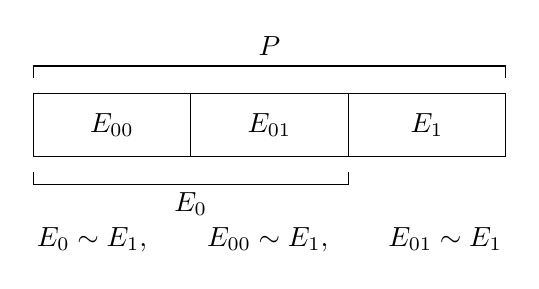
\begin{tikzpicture}[x=1cm,y=1cm]
\draw (0,0) rectangle (6,0.8);
\draw (2,0) -- (2,0.8);
\draw (4,0) -- (4,0.8);
\node at (1,0.4) {$E_{00}$};
\node at (3,0.4) {$E_{01}$};
\node at (5,0.4) {$E_1$};
\draw (0,1) -- (0,1.15) -- (6,1.15) -- (6,1);
\node at (3,1.4) {$P$};
\draw (0,-0.2) -- (0,-0.35) -- (4,-0.35) -- (4,-0.2);
\node at (2,-0.6) {$E_0$};
\node at (3,-1.05) {$E_0\sim E_1,\qquad E_{00}\sim E_1,\qquad E_{01}\sim E_1$};
\end{tikzpicture}
\caption{The decompositions $P=E_0+E_1$ and $E_0=E_{00}+E_{01}$,
shown schematically. The three disjoint cells are orthogonal; the
bracketed corner $E_0$ contains its two children. Here $\sim$ denotes
the equivalence in \eqref{eq:corner-equivalence}.}
\label{fig:kernel-corners}
\end{figure}

Fix $z\in\ker\pi$ and let $z_Q$ denote its image under the
coefficient map $a\mapsto\psi(a)Q$ for each of these idempotents.
Lemma~\ref{lem:corner-comparison}, applied three times with the
second corner $E_1$, gives
\begin{equation}\label{eq:four-corner-equality}
 z_{E_0}=z_{E_1}=z_{E_{00}}=z_{E_{01}}.
\end{equation}
By additivity, the second split in \eqref{eq:four-corner-splits}
splits every root image into its two child images.
Lemma~\ref{lem:orthogonal-root-images} permits their factors to be
collected separately in any word.  Hence
\[
 z_{E_0}=z_{E_{00}}z_{E_{01}}=z_{E_0}^{\,2},
\]
so $z_{E_0}=1$ and then $z_{E_1}=1$.
Finally $\psi(a)P=\psi(a)$.  The first split in
\eqref{eq:four-corner-splits}, with the same commutation argument,
therefore gives
\[
 \theta(z)=z_P=z_{E_0}z_{E_1}=1.
\]
\end{proof}

For $R=B\otimes_k B^{\mathrm{op}}$ and
$\psi=\phi\otimes\phi^{\mathrm{op}}$, the elements $P,U_i,V_i$
constructed in Section~\ref{sec:reduction} satisfy the support and
commutation hypotheses and the pair identities \eqref{eq:ring-pairs}.
Theorem~\ref{thm:kernel} therefore applies to the Steinberg transition
of Section~\ref{sec:affine}: it annihilates the matrix kernel in one step.
